\section{Verbesserungen des ersten Modells}
\label{chap:VerbesserungenNN}

In Kapitel \ref*{chap:DefineNN} wurde gezeigt, wie ein Modell für die Vorhersage für den Statuswert aussehen kann. Diese Schritte müssten ebenfalls für das dazugehörige Statement
durchlaufen werden. Das Ergebnis wären zwei unabhängige Modelle, die beide jeweils einzeln und nacheinander trainiert werden müssen. Diese Aufteilung ist nötig gewesen,
da die \glqq Sequential\grqq{}-Klasse es nicht erlaubt mehrere Ausgabeschichten zu definieren und da die \glqq softmax\grqq{}-Funktion allen Ausgabeneuronen 
einen Wert zuordnet, die addiert eins ergeben. Um dieses Problem zu umgehen, kann statt der \glqq Sequential\grqq{}-Klasse von Keras, die funktionale Keras-\ac{API} genutzt werden. 
Dadurch wird es ermöglicht Modelle zu definieren, die mehr als eine Eingabe- oder Ausgabeschicht haben oder Verzweigungen zwischen den Layern besitzen \cite[vgl. S.299f.]{DL_PY}. 
Abbildung \ref*{fig:FunktionaleAPI} zeigt den Aufbau eines \ac{NN} mit zwei Ausgabeschichten. Genau so ein Modell wird im nächsten Schritt mit der funktionalen Keras-\ac{API} erstellt.

\begin{figure}[H]
    \centering
    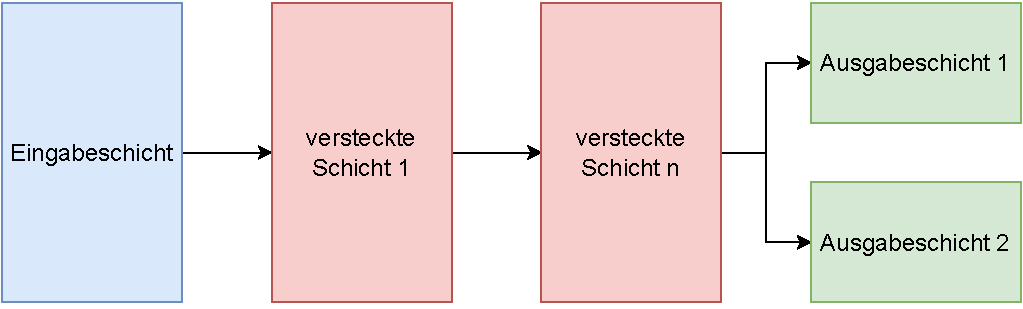
\includegraphics[width=\textwidth]{abbildungen/NN_funktionaleAPI.pdf}
    \caption{Modell mit zwei Ausgabeschichten}
    \label{fig:FunktionaleAPI}
\end{figure}

Grundsätzlich ist es möglich jedes Modell, welches mit der \glqq Sequential\grqq{}-Klasse erstellt wurde, in ein Modell mit der funktionalen Keras-\ac{API} zu übersetzen. 
Deshalb wird als Erstes das bestehende und in Kapitel \ref*{chap:DefineNN} beschriebene Modell übersetzt und im Anschluss daran wird dem Modell eine zweite Ausgabeschicht
hinzugefügt.
Mit der funktionalen \ac{API} werden Tensoren direkt bearbeitet und können den Schichten, wie bei einer Funktion, übergeben und entgegengenommen werden. Ziel dabei ist es 
aus einem Eingabetensor einen Ausgabetensor zu erzeugen. Dafür ruft die Bibliothek alle Schichten ab, die an dieser Transformation beteiligt sind und fasst diese Struktur
dann als Modell zusammen. Der Ausgabetensor entsteht also durch mehrere Transformationen des Eingabetensors \cite[vgl. S.305]{DL_PY}. 
Quellcode \ref*{lst:SeqToFunc} zeigt die Definition des Modells aus Kapitel \ref*{chap:DefineNN} mit der funktionalen \ac{API} und kann mit Quellcode \ref*{lst:ModellSeq}
verglichen werden. 

\begin{lstlisting}[language = python, caption={Modell mit funktionaler \acs{API} darstellen},captionpos=b, label = lst:SeqToFunc, floatplacement=H]
    input = Input(shape=(trainX.shape[1],))
    x = Dense(8, activation='relu')(input)
    x = Dense(16, activation='relu')(x)
    output = Dense(trainYStatus.shape[1], activation='softmax')(x)
    model = Model(input, output)
    model.summary()
    ---------------------------------------
    Output:
    ______________________________________________________________
    Layer (type)                Output Shape              Param #   
    ==============================================================
    input_9 (InputLayer)        [(None, 177)]             0         
                                                                    
    dense_36 (Dense)            (None, 8)                 1424      
                                                                    
    dense_37 (Dense)            (None, 16)                144       
                                                                    
    dense_38 (Dense)            (None, 3)                 51        
                                                                    
    ==============================================================
    Total params: 1,619
    Trainable params: 1,619
    Non-trainable params: 0
    ______________________________________________________________

\end{lstlisting}

Anders als bei der Erstellung des Modells mit der \glqq Sequential\grqq{}-Klasse, wird hier die Dimension der Eingabedaten nicht in der ersten Schicht als Parameter übergeben,
sondern wird noch vorher festgelegt. Wie in der Zusammenfassung des Modells jedoch zu sehen ist, stellt \glqq Input\grqq{} jedoch keine wirkliche erste Schicht dar,
da sie keine Parameter besitzt. Bis auf diesen Unterschied ist die Zusammenfassung beider Modelle gleich. Der Prozess des Trainierens und die Auswahl der Verlustfunktion
sowie des Optimierers sind ebenfalls identisch. Deshalb sind beide Modelle in der Anwendung äquivalent. Nun muss noch eine weitere zusätzliche Ausgabeschicht hinzugefügt werden,
welche das Statement zur Bewertung der Anwendungsregel prognostizieren soll. Dafür werden Zeile vier und fünf des Quellcodes \ref*{lst:SeqToFunc} überarbeitet, was 
in Quellcode \ref*{lst:Outputs} gezeigt wird.

\begin{lstlisting}[language = python, caption={Zweite Ausgabeschicht hinzufügen},captionpos=b, label = lst:Outputs, floatplacement=H]
    output1 = Dense(trainYStatus.shape[1], activation='softmax', name='status')(x)
    output2 = Dense(trainYStatement.shape[1], activation='softmax', name='statement')(x)
    model = Model(inputs=input, outputs=[output1, output2])
\end{lstlisting}

Beide Ausgabeschichten erhalten als Parameter die Anzahl an möglichen Ausprägungen ihres Zielattributs sowie eine Aktivierungsfunktion. An dieser Stelle wäre es möglich
auch verschiedene Aktivierungsfunktionen auszuwählen, sollte beispielsweise ein Zielattribut das Ergebnis einer Regression sein, könnte hier auch 
\glqq mse\grqq{} gewählt werden. Zudem erhalten die beiden Layer noch einen eindeutigen Namen. Beim Aufruf der compile()-Methode besteht dadurch die Möglichkeit 
den beiden Schichten unterschiedliche Verlustfunktionen zuzuweisen \cite[vgl. S.308f.]{DL_PY}. Da beide Layer hier jedoch eine Single-Label-Mehrfachklassifizierung lösen sollen,
wird das nicht benötigt. 

Das Übersetzen der beiden Modelle mit der \glqq Sequential\grqq{}-Klasse in ein Modell mit der funktionalen \ac{API} hat den Vorteil, dass nun nur noch ein Modell 
erstellt und trainiert werden muss, was die Laufzeit des Modells halbiert und zudem Zeilen an Code spart. 